% \documentclass[handout]{beamer}
\documentclass{beamer}

%%
%%
%%
% From http://tex.stackexchange.com/questions/2072/beamer-navigation-circles-without-subsections
% Solution #2 or 3:
% \usepackage{etoolbox}
% \makeatletter
% % replace the subsection number test with a test that always returns true
% \patchcmd{\slideentry}{\ifnum#2>0}{\ifnum2>0}{}{\@error{unable to patch}}%
% \makeatother
% Solution #1:
\usepackage{remreset}% tiny package containing just the \@removefromreset command
\makeatletter
\@removefromreset{subsection}{section}
\makeatother
\setcounter{subsection}{1}


\usepackage{etex}
\usepackage{pgf}
\usepackage{tikz}
\usepackage{url}
\usepackage{amsmath}
\usepackage{color}
% \definecolor{red}{rgb}{1,0,0}
\usepackage{ulem}
% \usepackage{booktabs}
\usepackage{colortbl,booktabs}
\renewcommand*{\thefootnote}{\fnsymbol{footnote}}
\usepackage{fancybox}
\usepackage[framemethod=TikZ]{mdframed}
\mdfdefinestyle{FactStyle}{%
  outerlinewidth=0.5,
  roundcorner=1pt,
  leftmargin=1cm,
  linecolor=blue,
  outerlinecolor=blue!70!black,
  backgroundcolor=yellow!40
}
\usepackage{cancel}

  \newcommand\Warning{%
    \makebox[2.4em][c]{%
      \makebox[0pt][c]{\raisebox{.2em}{\Large!}}%
      \makebox[0pt][c]{\color{red}\Huge$\bigtriangleup$}}}%

\usepackage{stackengine}
\usepackage{scalerel}
\usepackage{xcolor}
  \newcommand\dangersign[1][2ex]{%
    \renewcommand\stacktype{L}%
    \scaleto{\stackon[1.3pt]{\color{red}$\triangle$}{\tiny !}}{#1}%
  }



\usepackage{dcolumn}
\newcolumntype{d}[1]{D{.}{.}{#1}}

% From
% http://tex.stackexchange.com/questions/109900/how-can-i-box-multiple-aligned-equations
\usepackage{empheq}
\usepackage{tcolorbox}  \newtcbox{\othermathbox}[1][]{%
  nobeforeafter, tcbox raise base, 
  colback=black!10, colframe=red!30, 
  left=1em, top=0.5em, right=1em, bottom=0.5em}

\newcommand\blue{\color{blue}}
\newcommand\red{\color{red}}
\newcommand\green{\color{green!75!black}}
\newcommand\purple{\color{purple}}
\newcommand\bluegreen{\color{blue!75!green}}
\newcommand\orange{\color{orange}}
\newcommand\redgreen{\color{red!50!green}}
\newcommand\grey{\color{black}}
\newcommand\gap{\vspace{.1in}}
\newcommand\nb{${\red\bullet}\ $}
\newcommand\halfgap{\vspace{.05in}}
\newcommand\divideline{\line(1,0){352}}
\usepackage{marvosym} % for \Smiley

\newcommand{\bluealert}[1]{{\blue\textbf{#1}}}

% \usepackage{beamerthemesplit} %Key package for beamer
\usetheme{Singapore}
% \usetheme{Szeged}
% \usetheme{Garfield}
% \usetheme{CambridgeUS}
% \usenavigationsymbolstemplate{} %Gets rid of slide navigation symbols


\setbeamercolor{separation line}{use=structure,bg=structure.fg!50!bg}
% \begin{beamercolorbox}[colsep=0.5pt]
%   {upper separation line foot}
% \end{beamercolorbox}



\makeatletter
\setbeamertemplate{footline}
{
  \leavevmode%
  \hbox{%
% \begin{beamercolorbox}[colsep=0.5pt]
%   {upper separation line foot}
% \end{beamercolorbox}


  \begin{beamercolorbox}[wd=.5\paperwidth,ht=2.25ex,dp=2ex,colsep=0.5pt]%
    {upper separation line foot}
    \usebeamerfont{author in head/foot}%
    \hspace*{2ex}\insertshortdate:\ \insertshorttitle
  \end{beamercolorbox}%
  \begin{beamercolorbox}[wd=.5\paperwidth,ht=2.25ex,dp=2ex,right]{title in head/foot}%
    \usebeamerfont{title in head/foot}
    {\insertshortauthor}\hspace*{2ex}
  \end{beamercolorbox}}%
  % \begin{beamercolorbox}[wd=.333333\paperwidth,ht=2.25ex,dp=2ex,right]{date in head/foot}%
  %   \usebeamerfont{date in head/foot}\insertshortdate{}\hspace*{2em}
  %   \insertframenumber{} / \inserttotalframenumber\hspace*{2ex} 
  % \end{beamercolorbox}%
  \vskip0pt%
}
\makeatother

\usetikzlibrary{decorations.markings}
\usetikzlibrary{arrows}


\title{Final Exam Review}
\author{Peter Garfield, UCSB Mathematics}
\date{March 15, 2017}
%\institute{}


\useinnertheme{default}

\usefonttheme{serif}
% \usecolortheme{rose}
% \usecolortheme{whale}
% \usecolortheme{orchid}
\usecolortheme{crane}
% \usecolortheme{dolphin}


%TEMPLATE
\setbeamertemplate{navigation symbols}{}

\setbeamertemplate{note page}[compress]

\setbeamertemplate{frametitle}{
  \vspace{0.5em}
  % \begin{centering}
  {\huge\blue\textbf{\textmd{\insertframetitle}}}
  \par
  % \end{centering}
}

% From http://tex.stackexchange.com/questions/7032/good-way-to-make-textcircled-numbers:
\newcommand*\circled[1]{\tikz[baseline=(char.base)]{\node[shape=circle,draw,fill=orange,inner sep=1pt] (char) {#1};}} 
% \renewcommand{\labelenumi}{\circled{\textbf{\arabic{enumi}}}}

\let\olddescription\description
\let\oldenddescription\enddescription
\usepackage{enumitem}
\let\description\olddescription
\let\enddescription\oldenddescription

% \usepackage[loadonly]{enumitem}
\setlist[enumerate,1]{label=\colorbox{orange}{\arabic*.},font=\bfseries}
%\setlist[enumerate,2]{label=\colorbox{blue!25}{(\alph*)},font=\bfseries}
% \setlist[enumerate,1]{label=\arabic*.,font=\bfseries}
\setlist[itemize,1]{label=\red$\bullet$}
\setlist[itemize,2]{label=\blue$\bullet$}

\newcommand\answer[1]{\fbox{#1}}
% \renewcommand\answer[1]{}

\newcommand{\antilog}{\operatorname{antilog}}







\title{}
\title{Final Exam Review}
\date{June 9, 2017}


\begin{document}
\small

\section*{Administration}

\frame{
  \frametitle{Office Hours!}
  % \ \vspace*{0.25in}

  {\Large{}Instructor:}\\
  \ \hspace*{0.2in} Peter M.\ Garfield, \url{garfield@math.ucsb.edu}\\
  \ \hspace*{0.2in} South Hall 6510
  \vspace*{0.25in}
  \bigskip

  {\Large{}Office Hours:}\\
  \ \hspace*{0.2in} Monday: TBA \\
  \ \hspace*{0.2in} Tuesday: TBA \\
  \bigskip
  \vspace*{0.25in}

  {\Large{}Final Exam:}\\
  \ \hspace*{0.2in} Wednesday: 4:00--7:00\textsc{pm}
  \bigskip
  \vspace*{0.25in}

  \copyright\ 2017\ Daryl Cooper, Peter M.\ Garfield

  % \vspace*{2in}
}

\section{HW / Exam Problems}

\frame{
  \frametitle{HW 23 Problem \#4}

  A commuter railway has 800 passengers per day and charges each one
  two dollars per day. For each $4$ cents that the fare is increased, $5$
  fewer people will go by train. What is the greatest profit that can
  be earned?
  \bigskip

  \uncover<2->{``Profit'' in this case must mean ``Revenue''}
  \vspace*{2in}



}

\frame{
  \frametitle{W '14 Problem \#9}

    Carol's chocolate cookies cost \$$2$\ each and she sells
    $2200$ at this price. For each cent she raises the price she sells 
    $5$ fewer cookies. The ingredients for $10$ cookies cost \$$2$. 

     If Carol increases the price of a cookie by $x$ cents:
    \begin{enumerate}
      \item[\colorbox{blue!50}{(a)}]
        How many cookies will she sell?
        \bigskip


      \item[\colorbox{blue!50}{(b)}]
        How many dollars profit does she make on each cookie? 
        \bigskip
      
      \item[\colorbox{blue!50}{(c)}]
        Express the total profit (in \$) in terms of $x$.
        \bigskip
      
      \item[\colorbox{blue!50}{(d)}]
        What should $x$ be to make the most profit?
        \bigskip
      
      \item[\colorbox{blue!50}{(e)}]
        What should the price in \$ of one cookie be to make the most profit?
        \bigskip
      
    \end{enumerate}  

}


\frame{
  \frametitle{W '15 Problem \#8}

  Let $f(x) = 20\sqrt{x}$.
  \begin{enumerate}
    \item[\red(a)] Find $f'(4)$. \\
      {}[Simplify your answer to something like $7/3$.]
      \bigskip

    \item[\red(b)] Find the tangent line approximation to $y=f(x)$ at $x=4$. 
      \bigskip

    \item[\red(c)] Use this to approximate the value of $20\sqrt{5}$.

    \end{enumerate}
    \vspace*{2in}

}


\frame{
  \frametitle{W '15 Problem \#3(c)}

  Compute $\displaystyle\frac{d}{dx} \Big( (3x^2+5)/x^k \Big)$. 
  \smallskip

  [Here $k$ is a constant.]

  \vspace*{3in}

}

\section{Rates Of Change}

\frame{
  \frametitle{Review: Rates of Change}

  {\red(1)} Suppose $f(x) = x^2-x$. 
  \smallskip

  {\blue(a)}\ What is the average rate of change of $f(x)$ between
  $x=1$ and $x=3$?
  \vspace*{-0.5em}
  \begin{center}
    A $=1$
    \quad 
    B $=2$
    \quad 
    C $=3$
    \quad 
    D $=4$
    \quad 
    E $=5$
    \pause
    \quad
    \fbox{C}
  \end{center}

  {\blue(b)}\ What is the instantaneous rate of change of $f(x)$ at $x=3$?
  \begin{center}
    A $=1$
    \quad 
    B $=2$
    \quad 
    C $=3$
    \quad 
    D $=4$
    \quad 
    E $=5$
    \pause
    \quad
    \fbox{E}
  \end{center}
  % \bigskip
  \pause

  \begin{minipage}{0.65\linewidth}
    {\red(2)}\ The table to the right shows the number total number of
    people treated in a hospital up to and including the day shown
    during a flu outbreak.
  \end{minipage}
  \begin{minipage}[t]{0.3\linewidth}
    \begin{tabular}{|l||l|l|l|l|l|l|}\hline
      days & 0 & 3 & 7 & 9 \\
      \hline
      cases & 0 & 18 & 56 & 81 \\
      \hline
    \end{tabular}    
  \end{minipage}
  \smallskip

  {\blue(a)}\ On average, how many people were treated per day during the first week?
  \begin{center}
    A $=56$
    \quad 
    B $= 38$
    \quad 
    C $= 81$
    \quad 
    D $= 8$
    \pause
    \quad
    \fbox{D}
  \end{center}

  {\blue(b)}\ Which period had the greatest average number of cases per day?
  \begin{center}
    A $=0-3$ 
    \quad 
    B $= 3-7$
    \quad 
    C $= 7-9$
    \pause
    \quad
    \fbox{C}
  \end{center}


}




\frame{
  \frametitle{Jason \& Marie}

  \begin{itemize}
  \item Jason Bourne and Marie Kreutz are $270$ miles apart at noon.

  \item Marie drives towards Jason at constant speed $M$ starting at
    noon. 

  \item Jason sets out at $2$pm driving towards Marie at constant speed
    $J$. 

  \item They meet at $4$pm. 

  \end{itemize}

  {\red(1)}\ Which of the following equations is true?
  \begin{center}
    A\ \ $J+M=270$
    \quad 
    B\ \ $2J=4M$
    \quad 
    C\ \ $J-M=270$\\[0.5em]
    \ 
    \quad
    D\ \ $2J+4M=270$
    \quad 
    E\ \ $2J=270+4M$
    \quad
    \pause
    \fbox{D}
  \end{center}
  \pause
  \begin{itemize}
  \item At $3$pm, they are $100$ miles apart. 
  \end{itemize}

  {\red(2)}\ Which of the following equations is true?\\
  \begin{center}
    A\ \ $J+M=100$
    \quad 
    B\ \ $2J=4M$
    \quad 
    C\ \ $J-M=100$\\[0.5em]
    D\ \ $2J+4M=100$
    \quad 
    E\ \ $2J=100+4M$
    \quad
    \pause
    \fbox{A}
  \end{center}
  \vspace*{2.5in}



}



\frame{
  \frametitle{Jason \& Marie (continued)}

  \begin{itemize}
  \item Jason Bourne and Marie Kreutz are $270$ miles apart at noon.

  \item Marie drives towards Jason at constant speed $M$ starting at
    noon. 

  \item Jason sets out at $2$pm driving towards Marie at constant speed
    $J$. 

  \item They meet at $4$pm. 

  \item At $3$pm, they are $100$ miles apart. 
  \end{itemize}

  {\red(3)}\ What was Jason's speed ?
  \begin{center}
    A $= 35$
    \quad 
    B $= 45$
    \quad 
    C $= 55$
    \quad 
    D $= 65$
    \quad 
    E $= 75$
    \pause
    \quad
    \fbox{D}
  \end{center}
  \vspace*{4in}


}


\section{General Review}

\frame{

  \ \hspace*{-0.45in}
  \begin{minipage}{0.6\linewidth}
    \begin{center}
      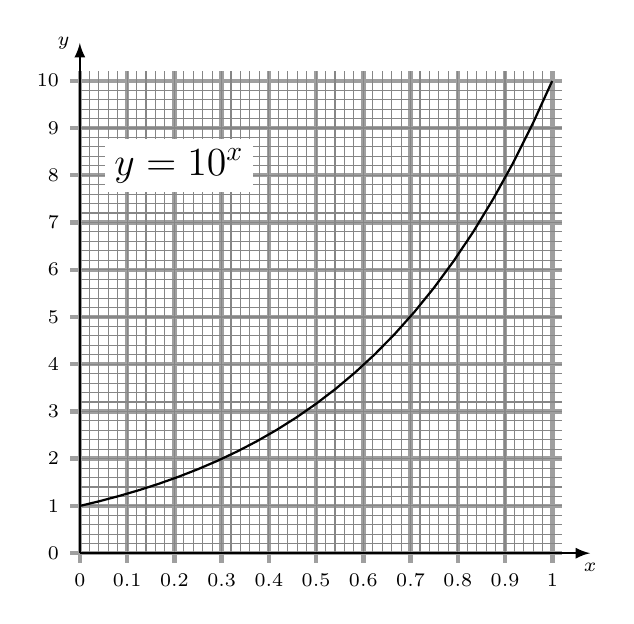
\begin{tikzpicture}[x=60mm,y=6mm,>=latex]
        \foreach \x in {0,0.1,0.2,0.3,0.4,0.5,0.6,0.7,0.8,0.9,1}
        {
          \draw[ultra thick,gray!75] (\x,10.2) -- (\x,-0.2) node[black,below] {$\scriptstyle\x$};
        }
        \foreach \y in {0,1,...,10} 
        {
          \draw[ultra thick,gray!75] (1.02,\y) -- (-0.02,\y) node[black,left] {$\scriptstyle\y$};
        }
        \foreach \k in {2,4,...,98}
        {
          \draw[thin,gray!95] ({\k/100},10.2) -- ({\k/100},0);
          \draw[thin,gray!95] (1.02,{\k/10}) -- (0,{\k/10});
        }
        % 
        \draw[thick,black,->] (0,0) -- (1.08,0) node[below] {$\scriptstyle{}x$};
        \draw[thick,black,->] (0,0) -- (0,10.8) node[left] {$\scriptstyle{}y$};
        \draw[thick,black] plot[domain=0:1] (\x,{10^(\x)});
        \node[black,fill=white] at (0.21,8.2) {\Large$y=10^x$};
      \end{tikzpicture}
    \end{center}
  \end{minipage}
  \hspace*{0.35in}
  \begin{minipage}{0.35\linewidth}
    Use the graph of $y=10^x$ to find:
    \begin{itemize}
    \item[(A)] $10^{3.65}$
      
      \uncover<2->{\alert{Answer:}\ $4500$}

    \item[(B)] Solve $10^x =73$

      \uncover<3->{\alert{Answer:}\ $1.86$}

    \item[(C)] The slope of the graph at $x=0.65$

      \uncover<4->{\alert{Answer:}\ $10$}

    \item[(D)] The average rate of change of $10^x$ between $x=0.1$
      and $x=0.6$ 

      \uncover<5->{\alert{Answer:}\ $5$}

    \end{itemize}


    
  \end{minipage}




}


\frame{
  \frametitle{Review: Lines!}

  \begin{enumerate}
    \setcounter{enumi}{0}
  \item Find the equation of the line with slope $3$ that contains the
    point $(2,5)$.
    \begin{center}
      A\ $y = 3x+5$
      \quad 
      B\ $y=3x-1$
      \quad 
      C\ $y =3x + 2$
      \pause
      \quad
      \fbox{B}
    \end{center}
    \bigskip

    \item What is the $x$-coordinate of the point where the two lines 
      \begin{equation*}
        y= 3x+2
        \qquad\text{and}\qquad
        y - 4x+1=0
      \end{equation*}
      cross?
      \begin{center}
        A\ $x=-3$
        \quad 
        B\ $x=-1$
        \quad 
        C\ $x=1$
        \quad
        D\ $x=3$
        \quad 
        E\ $x=4$
        \pause
        \quad
        \fbox{D}
      \end{center}
      \bigskip

      % \item Find the equation of the tangent line to $y=2x^3-2x$ at $x=1$.
      % \begin{center}
      %   A\ $y=2x-6$
      %   \quad 
      %   B\ $y=16x-7$
      %   \quad 
      %   C\ $y = 7x+16$
      %   \quad 
      %   D\ $y = 7x-16$
      %   \pause
      % \end{center}

  \end{enumerate}

}

\frame{
  \frametitle{Review: Logs!}

  \begin{enumerate}
    \setcounter{enumi}{2}
  \item Solve $3^x=7$.
    \begin{center}
      A\ $x= 7/3$
      \quad 
      B\ $x=\log(7/3)$
      \\
      \ \quad
      C\ $x =\log(7)/\log(3)$
      \quad 
      D\ $x = \log(7)-\log(3)$
      \pause
      \quad
      \fbox{C}
    \end{center}
    \vspace*{-1em}


    \ \hspace*{-0.5in}
    \begin{minipage}[t]{0.35\linewidth}
      \bluealert{Remember half-life}:\ 
    \end{minipage}
    \begin{minipage}[t]{0.65\linewidth}
      \begin{itemize}
      \item Half-life $=K$ years 
      \item Initial amount $=A$
      \item Amount after $t$ years is \fbox{$=A \times 2^{-t/K}$}
      \end{itemize}
    \end{minipage}
    % \bigskip

  \item Let's start with $8$ grams of an element with half-life of $5$
    years.

    {\red(a)}\ How many grams remain after $10$ years?
    \begin{center}
      A\ $= 0$
      \quad 
      B\ $=2$
      \quad 
      C\ $= 4$
      \quad 
      D\ $=8$
      \pause
      \quad
      \fbox{B}
    \end{center}
    % \smallskip

    {\red(b)}\ How many years until $3$ grams remain?
    \begin{center}
      A\ $= 8/3$
      \quad 
      B\ $= -5\log(3/8)/\log(2)$
      \\[0.5em] 
      \ 
      \quad 
      C\ $=-5\log(3/16)$
      \ \quad 
      D\ $= \log(3/8)-\log(2)$
      \pause
      \quad
      \fbox{B}
    \end{center}

  \end{enumerate}
}


\end{document}
\frame{
  \frametitle{Review: Rates of Change}

  {\red(1)} Suppose $f(x) = x^2-x$. 
  \smallskip

  {\blue(a)}\ What is the average rate of change of $f(x)$ between
  $x=1$ and $x=3$?
  \vspace*{-0.5em}
  \begin{center}
    A $=1$
    \quad 
    B $=2$
    \quad 
    C $=3$
    \quad 
    D $=4$
    \quad 
    E $=5$
    \pause
    \quad
    \fbox{C}
  \end{center}

  {\blue(b)}\ What is the instantaneous rate of change of $f(x)$ at $x=3$?
  \begin{center}
    A $=1$
    \quad 
    B $=2$
    \quad 
    C $=3$
    \quad 
    D $=4$
    \quad 
    E $=5$
    \pause
    \quad
    \fbox{E}
  \end{center}
  % \bigskip
  \pause

  \begin{minipage}{0.65\linewidth}
    {\red(2)}\ The table to the right shows the number total number of
    people treated in a hospital up to and including the day shown
    during a flu outbreak.
  \end{minipage}
  \begin{minipage}[t]{0.3\linewidth}
    \begin{tabular}{|l||l|l|l|l|l|l|}\hline
      days & 0 & 3 & 7 & 9 \\
      \hline
      cases & 0 & 18 & 56 & 81 \\
      \hline
    \end{tabular}    
  \end{minipage}
  \smallskip

  {\blue(a)}\ On average, how many people were treated per day during the first week?
  \begin{center}
    A $=56$
    \quad 
    B $= 38$
    \quad 
    C $= 81$
    \quad 
    D $= 8$
    \pause
    \quad
    \fbox{D}
  \end{center}

  {\blue(b)}\ Which period had the greatest average number of cases per day?
  \begin{center}
    A $=0-3$ 
    \quad 
    B $= 3-7$
    \quad 
    C $= 7-9$
    \pause
    \quad
    \fbox{C}
  \end{center}


}




\frame{
  \frametitle{Jason \& Marie}

  \begin{itemize}
  \item Jason Bourne and Marie Kreutz are $270$ miles apart at noon.

  \item Marie drives towards Jason at constant speed $M$ starting at
    noon. 

  \item Jason sets out at $2$pm driving towards Marie at constant speed
    $J$. 

  \item They meet at $4$pm. 

  \end{itemize}

  {\red(1)}\ Which of the following equations is true?
  \begin{center}
    A\ $J+M=270$
    \quad 
    B\ $2J=4M$
    \quad 
    C\ $J-M=270$\\[0.5em]
    \ 
    \quad
    D\ $2J+4M=270$
    \quad 
    E\ $2J=270+4M$
    \quad
    \pause
    \fbox{D}
  \end{center}
  \pause
  \begin{itemize}
  \item At $3$pm, they are $100$ miles apart. 
  \end{itemize}

  {\red(2)}\ Which of the following equations is true?\\
  \begin{center}
    A\ $J+M=100$
    \quad 
    B\ $2J=4M$
    \quad 
    C\ $J-M=100$\\[0.5em]
    D\ $2J+4M=100$
    \quad 
    E\ $2J=100+4M$
    \quad
    \pause
    \fbox{A}
  \end{center}
  \vspace*{2.5in}



}



\frame{
  \frametitle{Jason \& Marie (continued)}

  \begin{itemize}
  \item Jason Bourne and Marie Kreutz are $270$ miles apart at noon.

  \item Marie drives towards Jason at constant speed $M$ starting at
    noon. 

  \item Jason sets out at $2$pm driving towards Marie at constant speed
    $J$. 

  \item They meet at $4$pm. 

  \item At $3$pm, they are $100$ miles apart. 
  \end{itemize}

  {\red(3)}\ What was Jason's speed ?
  \begin{center}
    A $= 35$
    \quad 
    B $= 45$
    \quad 
    C $= 55$
    \quad 
    D $= 65$
    \quad 
    E $= 75$
    \pause
    \quad
    \fbox{D}
  \end{center}
  \vspace*{4in}


}


\frame{

  \ \hspace*{-0.45in}
  \begin{minipage}{0.6\linewidth}
    \begin{center}
      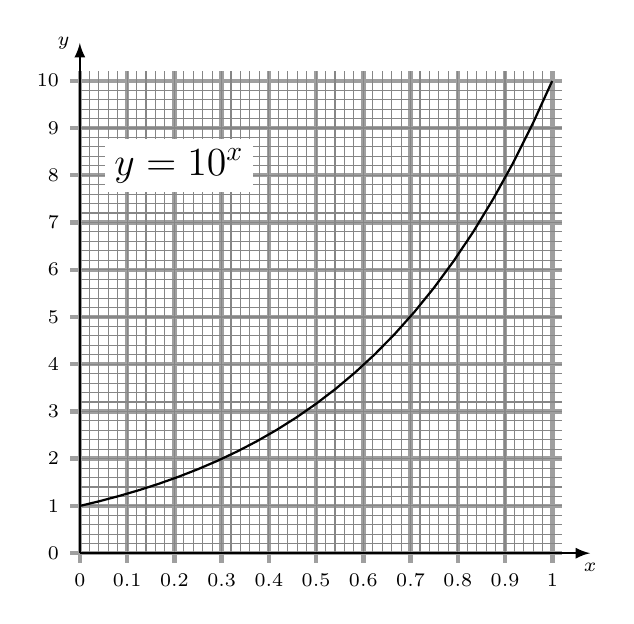
\begin{tikzpicture}[x=60mm,y=6mm,>=latex]
        \foreach \x in {0,0.1,0.2,0.3,0.4,0.5,0.6,0.7,0.8,0.9,1}
        {
          \draw[ultra thick,gray!75] (\x,10.2) -- (\x,-0.2) node[black,below] {$\scriptstyle\x$};
        }
        \foreach \y in {0,1,...,10} 
        {
          \draw[ultra thick,gray!75] (1.02,\y) -- (-0.02,\y) node[black,left] {$\scriptstyle\y$};
        }
        \foreach \k in {2,4,...,98}
        {
          \draw[thin,gray!95] ({\k/100},10.2) -- ({\k/100},0);
          \draw[thin,gray!95] (1.02,{\k/10}) -- (0,{\k/10});
        }
        % 
        \draw[thick,black,->] (0,0) -- (1.08,0) node[below] {$\scriptstyle{}x$};
        \draw[thick,black,->] (0,0) -- (0,10.8) node[left] {$\scriptstyle{}y$};
        \draw[thick,black] plot[domain=0:1] (\x,{10^(\x)});
        \node[black,fill=white] at (0.21,8.2) {\Large$y=10^x$};
      \end{tikzpicture}
    \end{center}
  \end{minipage}
  \hspace*{0.35in}
  \begin{minipage}{0.35\linewidth}
    Use the graph of $y=10^x$ to find:
    \begin{itemize}
    \item[(A)] $10^{3.65}$
      
      \uncover<2->{\alert{Answer:}\ $4500$}

    \item[(B)] Solve $10^x =73$

      \uncover<3->{\alert{Answer:}\ $1.86$}

    \item[(C)] The slope of the graph at $x=0.65$

      \uncover<4->{\alert{Answer:}\ $10$}

    \item[(D)] The average rate of change of $10^x$ between $x=0.1$
      and $x=0.6$ 

      \uncover<5->{\alert{Answer:}\ $5$}

    \end{itemize}


    
  \end{minipage}




}











\end{document}
